\documentclass[11pt]{article}
\usepackage{graphicx}
\usepackage{amsmath}
\usepackage{amsfonts}
\usepackage{natbib}
\usepackage{hyperref}
\usepackage{geometry}
\usepackage{enumitem}
\usepackage{booktabs}
\geometry{a4paper, margin=1in}

\begin{document}

\title{Analysis of Pulsar Timing Residuals for Gravitational Wave Background Detection: A Detailed Mathematical Perspective}
\author{}
\date{April 2025}
\maketitle

\begin{abstract}
This report provides a comprehensive mathematical analysis of pulsar timing residuals to detect a stochastic gravitational wave background (GWB) using a dataset of 20 pulsars observed over 16 years. The timing residuals are modeled as a combination of a GWB signal, an Earth-term signal, pulsar-specific red noise, white noise, and glitch/dispersion measure (DM) variations. We employ a differential evolution optimization algorithm to estimate the parameters of the GWB, Earth-term, and red noise, while fitting glitch and DM models for each pulsar. This document is designed for a mathematical audience, providing a detailed, step-by-step progression of the problem, including extensive mathematical derivations (e.g., Cholesky decomposition, likelihood function, antenna response functions, broken power law spectrum, Fourier transform of the glitch model), a rigorous statistical analysis of the residuals, and an exploration of alternative noise models. Technical terms such as the quadrupolar nature of gravitational waves, red noise, and dispersion measure are defined to bridge the gap between astrophysics and mathematics.
\end{abstract}

\section{Introduction}
Pulsar timing arrays (PTAs) are a powerful tool for detecting low-frequency gravitational waves, particularly the stochastic gravitational wave background (GWB) produced by supermassive black hole binaries \citep{ipta2013}. The GWB manifests as a correlated signal in the timing residuals of millisecond pulsars, characterized by a specific angular correlation known as the Hellings-Downs curve \citep{hellings1983}. However, pulsar timing residuals also contain contributions from other astrophysical and instrumental effects, such as pulsar-specific red noise, white noise, glitches, and dispersion measure (DM) variations due to the interstellar medium.

This analysis aims to:
\begin{enumerate}
    \item Detect and characterize the GWB by estimating its amplitude ($A_{gw}$) and spectral index ($\gamma$).
    \item Model an Earth-term signal, a common red noise process affecting all pulsars, with amplitude $A_{earth}$ and spectral index $\gamma_{earth}$.
    \item Estimate pulsar-specific red noise parameters ($A_{red,i}$, $\gamma_{red,i}$) for each of the 20 pulsars.
    \item Fit glitch and DM variations for each pulsar, with a focus on Pulsar 20, which exhibits a distinct glitch signature.
\end{enumerate}

This document is tailored for a mathematical audience, providing a detailed progression from the astrophysical problem to the mathematical solution. We assume familiarity with linear algebra, Fourier analysis, optimization, and statistical methods, but we provide introductions to astrophysical concepts and define technical terms to ensure clarity. The document includes extensive mathematical derivations, a rigorous statistical analysis, and an exploration of alternative models.

\section{Background: Pulsars and Gravitational Waves}

\subsection{What Are Pulsars?}
Pulsars are rapidly rotating neutron stars—extremely dense remnants of massive stars that have undergone a supernova explosion—that emit beams of radio waves from their magnetic poles. As the pulsar rotates, these beams sweep across the Earth, producing periodic pulses of radio emission, much like a lighthouse. Millisecond pulsars, with rotation periods on the order of milliseconds, are particularly stable and can be used as precise astrophysical clocks \citep{lorimer2008}.

The arrival times of these pulses, known as times of arrival (TOAs), are measured with high precision using radio telescopes. The timing residuals are defined as the difference between the observed TOAs and the predicted TOAs based on a model of the pulsar’s rotation, position, and motion:
\[
r(t) = t_{\text{observed}} - t_{\text{predicted}}.
\]
These residuals contain contributions from various physical effects, including gravitational waves, noise processes, and pulsar-specific phenomena like glitches (sudden changes in rotation frequency).

\subsection{Gravitational Waves and the Stochastic GWB}
Gravitational waves are ripples in spacetime caused by the acceleration of massive objects, such as binary systems of supermassive black holes. When a gravitational wave passes between a pulsar and the Earth, it perturbs the spacetime metric, causing a small change in the proper distance and thus a delay or advance in the pulse arrival time. The stochastic GWB is a superposition of gravitational waves from many unresolved sources, primarily supermassive black hole binaries in the early universe \citep{phinney2001}. The GWB produces a red noise signal in the timing residuals, with a power-law spectrum:
\[
P_{gw}(f) = \frac{A_{gw}^2}{12 \pi^2} \left( \frac{f}{f_{yr}} \right)^{-\gamma},
\]
where $A_{gw}$ is the amplitude, $\gamma$ is the spectral index, $f$ is the frequency, and $f_{yr} = 1/\text{year}$ is the reference frequency (approximately $3.17 \times 10^{-8}$ Hz for a year-long period). A \textit{power-law spectrum} means that the power $P(f)$ scales as a power of the frequency $f$, i.e., $P(f) \propto f^{-\gamma}$. \textit{Red noise} refers to a noise process where the power is concentrated at low frequencies (large $\gamma$), as opposed to \textit{white noise}, where the power is constant across all frequencies.

For a GWB produced by supermassive black hole binaries, the spectral index is expected to be $\gamma = 13/3 \approx 4.33$, based on theoretical models of binary evolution \citep{phinney2001}. The amplitude $A_{gw}$ is typically on the order of $10^{-15}$ to $10^{-14}$, reflecting the strain amplitude of the gravitational waves.

\subsection{The Hellings-Downs Correlation}
The GWB signal is unique because it induces a correlated signal across pairs of pulsars, with the correlation depending on the angular separation $\zeta$ between the pulsars. This correlation is described by the Hellings-Downs curve \citep{hellings1983}:
\[
\Gamma(\zeta) = \frac{3}{2} x \ln x - \frac{x}{4} + \frac{1}{2}, \quad x = \frac{1 - \cos \zeta}{2}.
\]
The Hellings-Downs curve arises from the \textit{quadrupolar nature} of gravitational waves. In general relativity, gravitational waves are transverse waves with two polarization states: the plus ($+$) and cross ($\times$) polarizations. These polarizations describe the way spacetime is stretched and compressed as the wave passes. The term "quadrupolar" refers to the fact that gravitational waves are generated by the second derivative of the mass quadrupole moment of a source (e.g., a binary system), and their effect on spacetime has a quadrupolar pattern—stretching in one direction while compressing in the perpendicular direction, with a 45-degree angular dependence between the two polarizations. The Hellings-Downs correlation is derived by averaging the gravitational wave strain over all possible source directions on the sky, taking into account the geometry of the pulsar pair relative to the wave’s propagation direction.

\section{Astrophysical Problem: A Mathematical Perspective}
The goal is to detect the stochastic GWB in the presence of other noise sources and pulsar-specific effects. Mathematically, the timing residuals for each pulsar $i$ can be written as:
\[
r_i(t) = r_{gw,i}(t) + r_{earth,i}(t) + r_{red,i}(t) + r_{white,i}(t) + r_{glitch/DM,i}(t),
\]
where:
\begin{itemize}
    \item $r_{gw,i}(t)$: The GWB signal, correlated across pulsars according to the Hellings-Downs curve.
    \item $r_{earth,i}(t)$: The Earth-term signal, a common red noise process affecting all pulsars.
    \item $r_{red,i}(t)$: Pulsar-specific red noise.
    \item $r_{white,i}(t)$: White noise, modeled as Gaussian noise.
    \item $r_{glitch/DM,i}(t)$: Glitch and DM variations, which are pulsar-specific.
\end{itemize}

The problem can be framed as a signal decomposition task:
\begin{enumerate}
    \item \textbf{Signal Separation}: Decompose the residuals into the GWB signal and other components.
    \item \textbf{Correlation Analysis}: Use the Hellings-Downs correlation to identify the GWB signal.
    \item \textbf{Parameter Estimation}: Estimate the parameters of each component using optimization techniques.
    \item \textbf{Statistical Validation}: Assess the significance of the GWB detection and the goodness of fit.
\end{enumerate}

\section{Data Description}
The dataset consists of timing residuals for 20 pulsars observed over 16 years, with 1000 time points per pulsar (after interpolation). The data includes:
\begin{itemize}
    \item \textbf{Times of Arrival (TOAs)}: A matrix $T \in \mathbb{R}^{20 \times 1000}$, where $T[i, t]$ is the time of the $t$-th observation for pulsar $i$.
    \item \textbf{Residuals}: A matrix $R \in \mathbb{R}^{20 \times 1000}$, where $R[i, t]$ is the timing residual for pulsar $i$ at time $T[i, t]$.
    \item \textbf{Uncertainties}: A matrix $\Sigma \in \mathbb{R}^{20 \times 1000}$, where $\Sigma[i, t]$ is the measurement uncertainty for the $t$-th observation of pulsar $i$.
    \item \textbf{Pulsar Positions}: A matrix $P \in \mathbb{R}^{20 \times 2}$, where $P[i, :]$ contains the right ascension and declination of pulsar $i$, used to compute angular separations $\zeta_{ij}$.
\end{itemize}

The residuals exhibit a variety of features:
\begin{itemize}
    \item Low-frequency trends, potentially due to the GWB or Earth-term signal.
    \item High-frequency oscillations, likely due to red noise or white noise.
    \item Sudden jumps or trends, such as glitches (e.g., Pulsar 20 shows a drop at 2 years) or DM variations.
\end{itemize}

The angular separations $\zeta_{ij}$ are computed using the spherical law of cosines:
\[
\cos \zeta_{ij} = \sin(\text{dec}_i) \sin(\text{dec}_j) + \cos(\text{dec}_i) \cos(\text{dec}_j) \cos(\text{ra}_i - \text{ra}_j),
\]
\[
\zeta_{ij} = \arccos(\cos \zeta_{ij}),
\]
where $\text{ra}_i$ and $\text{dec}_i$ are the right ascension and declination of pulsar $i$.

\section{Model Description}
We model the timing residuals as a combination of several components, each with its own mathematical form.

\subsection{GWB Signal}
The GWB signal is modeled as a red noise process with a power-law spectrum:
\[
P_{gw}(f) = \frac{A_{gw}^2}{12 \pi^2} \left( \frac{f}{f_{yr}} \right)^{-\gamma},
\]
where $f_{yr} = 1/(365.25 \times 86400) \approx 3.17 \times 10^{-8}$ Hz. The signal is generated in the frequency domain using the Fourier transform, with the power spectrum determining the amplitude of each frequency component. The GWB signal is correlated across pulsars according to the Hellings-Downs curve, as described in the Fourier domain modeling section.

\subsection{Earth-Term Signal}
The Earth-term signal is a common red noise process with a power-law spectrum:
\[
P_{earth}(f) = \frac{A_{earth}^2}{12 \pi^2} \left( \frac{f}{f_{yr}} \right)^{-\gamma_{earth}}.
\]
This signal is generated in the frequency domain and added to the residuals of all pulsars:
\[
r_{earth,i}(t) = r_{earth}(t), \quad \forall i.
\]

\subsection{Pulsar-Specific Red Noise}
Each pulsar has its own red noise process, with a power-law spectrum:
\[
P_{red,i}(f) = \frac{A_{red,i}^2}{12 \pi^2} \left( \frac{f}{f_{yr}} \right)^{-\gamma_{red,i}}.
\]
This signal is generated independently for each pulsar, allowing for different amplitudes and spectral indices.

\subsection{White Noise}
White noise is modeled as Gaussian noise with a standard deviation $\sigma_i$ for each pulsar $i$:
\[
r_{white,i}(t) \sim \mathcal{N}(0, \sigma_i / 8),
\]
where $\sigma_i$ is estimated from the standard deviation of the residuals, and the factor $1/8$ reduces the white noise contribution to allow the red noise components to dominate.

\subsection{Glitch and DM Variations}
A \textit{glitch} is a sudden increase in the pulsar’s rotation frequency, often followed by an exponential recovery, due to internal dynamics of the neutron star (e.g., superfluid interactions). \textit{Dispersion measure (DM)} variations refer to changes in the integrated electron density along the line of sight to the pulsar, which cause a frequency-dependent delay in the pulse arrival time due to the dispersive nature of the interstellar medium. The delay due to DM is proportional to $1/\nu^2$, where $\nu$ is the observing frequency.

For most pulsars, the glitch and DM model is:
\begin{align}
r_{glitch/DM,i}(t) &= \sum_{k=1}^{2} A_{glitch,k} \Theta(t - t_{glitch,k}) e^{-(t - t_{glitch,k})/\tau_{k}} + A_{DM} \Theta(t - t_{DM}) \notag \\
&\quad + s_{DM,1} (t - t_{DM}) \Theta(t_{glitch,2} - t) + s_{DM,2} (t - t_{glitch,2}) \Theta(t - t_{glitch,2}) \notag \\
&\quad + s_{global} t,
\end{align}
where $\Theta(t)$ is the Heaviside step function, defined as $\Theta(t) = 1$ for $t \geq 0$ and $\Theta(t) = 0$ for $t < 0$.

For Pulsar 20, we use a simplified model:
\[
r_{glitch,20}(t) = A_{glitch,2} \Theta(t - t_{glitch,2}) e^{-(t - t_{glitch,2})/\tau_{2}} + s_{global} t.
\]

\section{Fourier Domain Modeling}
The GWB, Earth-term, and red noise signals are generated in the Fourier domain, which is a natural choice for power-law spectra.

\subsection{Fourier Transform of the Residuals}
The timing residuals $r_i(t)$ are sampled at times $t_n = n \Delta t$, where $\Delta t$ is the time step, and $n = 0, 1, \ldots, 999$. The Fourier transform of the residuals is:
\[
\hat{r}_i(f_k) = \sum_{n=0}^{N-1} r_i(t_n) e^{-2\pi i f_k t_n}, \quad f_k = \frac{k}{N \Delta t}, \quad k = 0, 1, \ldots, N-1,
\]
where $N = 1000$. The inverse Fourier transform is:
\[
r_i(t_n) = \frac{1}{N} \sum_{k=0}^{N-1} \hat{r}_i(f_k) e^{2\pi i f_k t_n}.
\]

\subsection{Power Spectrum and Random Signal Generation}
For a red noise process with power spectrum $P(f)$, we generate the signal in the Fourier domain:
\[
\hat{r}(f_k) = \sqrt{P(f_k)} e^{i \phi_k}, \quad \phi_k \sim \text{Uniform}[0, 2\pi),
\]
where $P(f_k)$ is the power spectrum (e.g., $P_{gw}(f)$). The time-domain signal is:
\[
r(t_n) = \frac{1}{N} \sum_{k=0}^{N-1} \hat{r}(f_k) e^{2\pi i f_k t_n}.
\]

\subsection{Correlated GWB Signal}
For the GWB signal, we need to impose the Hellings-Downs correlation. The correlation matrix $C \in \mathbb{R}^{20 \times 20}$ is defined as:
\[
C_{ij} = \Gamma(\zeta_{ij}).
\]
We generate the Fourier coefficients for each pulsar:
\[
\hat{r}_{gw,i}(f_k) = \sqrt{P_{gw}(f_k)} \eta_i(f_k),
\]
where $\eta_i(f_k)$ are complex Gaussian random variables with the correlation $\langle \eta_i(f_k) \eta_j^*(f_k) \rangle = C_{ij}$. This is achieved using a Cholesky decomposition, as derived below.

\section{Parameters Being Estimated}
We estimate the following parameters:

\subsection{GWB and Earth-Term Parameters}
\begin{itemize}
    \item $A_{gw}$: Amplitude of the GWB, with bounds $[10^{-15}, 5 \times 10^{-15}]$.
    \item $\gamma$: Spectral index of the GWB, with bounds $[4, 5]$.
    \item $A_{earth}$: Amplitude of the Earth-term signal, with bounds $[5 \times 10^{-16}, 5 \times 10^{-15}]$.
    \item $\gamma_{earth}$: Spectral index of the Earth-term signal, with bounds $[2, 4]$.
\end{itemize}

\subsection{Pulsar-Specific Red Noise Parameters}
For each of the 20 pulsars:
\begin{itemize}
    \item $A_{red,i}$: Amplitude of the red noise, with bounds $[10^{-16}, 3 \times 10^{-15}]$.
    \item $\gamma_{red,i}$: Spectral index of the red noise, with bounds $[0.1, 1.5]$.
\end{itemize}

\subsection{Glitch and DM Parameters}
For each pulsar (except Pulsar 20):
\begin{itemize}
    \item $A_{glitch,1}$, $A_{glitch,2}$: Amplitudes of the two glitches, with bounds $[-10^{-5}, 10^{-5}]$ seconds.
    \item $t_{glitch,1}$, $t_{glitch,2}$: Times of the two glitches, with bounds $[0, 16]$ years.
    \item $\tau_{1}$, $\tau_{2}$: Decay timescales of the glitches, with bounds $[1, 365.25]$ days.
    \item $A_{DM}$: Amplitude of the DM step, with bounds $[-10^{-5}, 10^{-5}]$ seconds.
    \item $t_{DM}$: Time of the DM step, with bounds $[0, 16]$ years.
    \item $s_{DM,1}$, $s_{DM,2}$: DM slopes, with bounds $[-10^{-10}, 10^{-10}]$ s/s.
    \item $s_{global}$: Global linear trend, with bounds $[-10^{-10}, 10^{-10}]$ s/s.
\end{itemize}

For Pulsar 20:
\begin{itemize}
    \item $A_{glitch,2}$: Amplitude of the glitch, with bounds $[-10^{-5}, 0]$ seconds.
    \item $t_{glitch,2}$: Time of the glitch, with bounds $[1.9, 2.1]$ years.
    \item $\tau_{2}$: Decay timescale of the glitch, with bounds $[29, 31]$ days.
    \item $s_{global}$: Global linear trend, with bounds $[-10^{-14}, 10^{-14}]$ s/s.
\end{itemize}

\section{Optimization Process}
We use a two-step optimization process to fit the model to the data.

\subsection{Step 1: Glitch and DM Fitting}
For each pulsar, we fit the glitch and DM model by minimizing the sum of squared residuals:
\[
\text{Objective} = \sum_{t} \left( r_i(t) - r_{glitch/DM,i}(t) \right)^2.
\]
We use differential evolution to explore the parameter space, followed by least-squares optimization to refine the solution. The fitted model is subtracted from the residuals:
\[
r_i(t) \leftarrow r_i(t) - r_{glitch/DM,i}(t).
\]

\subsection{Step 2: GWB and Red Noise Fitting}
We fit the GWB, Earth-term, and red noise components using differential evolution. The fitness function is:
\[
\text{Fitness} = \chi^2 + \lambda \times \text{HD penalty}, \quad \lambda = 10^5.
\]
The $\chi^2$ term is:
\[
\chi^2 = \frac{1}{N_{pulsars} N_{times}} \sum_{i=1}^{N_{pulsars}} w_i \sum_{t} \left( \frac{r_i(t) - m_i(t)}{\sigma_i(t)} \right)^2,
\]
where $w_i$ are weights based on the number of non-NaN data points, and $m_i(t)$ is the model:
\[
m_i(t) = r_{gw,i}(t) + r_{earth,i}(t) + r_{red,i}(t) + r_{white,i}(t).
\]
The Hellings-Downs penalty term is:
\[
\text{HD penalty} = \sum_{i,j} \left( C_{ij} - \Gamma(\zeta_{ij}) \right)^2,
\]
where $C_{ij}$ is the correlation matrix of the GWB signal:
\[
C_{ij} = \frac{\sum_t \left( r_{gw,i}(t) - \bar{r}_{gw,i} \right) \left( r_{gw,j}(t) - \bar{r}_{gw,j} \right)}{N_{times} \sigma_{gw,i} \sigma_{gw,j}}.
\]

The differential evolution algorithm is run with a population size of 50 and a maximum of 300 iterations.

\section{Mathematical Derivations}

\subsection{Derivation of the GWB Power Spectrum}
The power spectrum of the GWB is derived from the characteristic strain $h_c(f)$:
\[
h_c(f) = A_{gw} \left( \frac{f}{f_{yr}} \right)^{\alpha}, \quad \alpha = -\frac{2}{3}.
\]
The spectral index $\gamma$ is related to $\alpha$ by:
\[
\gamma = 3 - 2\alpha.
\]
For $\alpha = -2/3$, we have $\gamma = 13/3 \approx 4.33$. The power spectrum of the timing residuals is:
\[
P_{gw}(f) = \frac{h_c(f)^2}{12 \pi^2 f^3} = \frac{A_{gw}^2}{12 \pi^2} \left( \frac{f}{f_{yr}} \right)^{2\alpha} f^{-3} = \frac{A_{gw}^2}{12 \pi^2} \left( \frac{f}{f_{yr}} \right)^{-\gamma}.
\]

\subsection{Derivation of the Hellings-Downs Correlation}
The Hellings-Downs correlation arises from the quadrupolar nature of gravitational waves. The strain $h(t)$ induced by a gravitational wave on a pulsar-Earth baseline is:
\[
h(t) = h_+(t) F_+ + h_\times(t) F_\times,
\]
where $h_+(t)$ and $h_\times(t)$ are the plus and cross polarizations, and $F_+$ and $F_\times$ are the antenna response functions, which depend on the geometry of the pulsar pair and the wave’s propagation direction. The timing residual is:
\[
r(t) = \int_{-\infty}^{t} h(t') \, dt'.
\]
The correlation between two pulsars is:
\[
\langle r_i(t) r_j(t) \rangle = \int_{-\infty}^{\infty} P_{gw}(f) F(\zeta) \, df,
\]
where $F(\zeta)$ is the angular response function, averaged over all source directions:
\[
F(\zeta) = \frac{3}{2} x \ln x - \frac{x}{4} + \frac{1}{2}, \quad x = \frac{1 - \cos \zeta}{2}.
\]

\subsection{Antenna Response Functions for the Hellings-Downs Correlation}
The antenna response functions $F_+$ and $F_\times$ describe how a gravitational wave affects the timing residuals of a pulsar. Consider a gravitational wave propagating in the direction $\hat{k}$, with the pulsar in the direction $\hat{p}$. The plus and cross polarizations are defined with respect to a coordinate system where the wave propagates along the $z$-axis, and the polarization axes are along the $x$- and $y$-axes. The strain tensor for the plus polarization is:
\[
h_+ \begin{pmatrix} 1 & 0 & 0 \\ 0 & -1 & 0 \\ 0 & 0 & 0 \end{pmatrix},
\]
and for the cross polarization:
\[
h_\times \begin{pmatrix} 0 & 1 & 0 \\ 1 & 0 & 0 \\ 0 & 0 & 0 \end{pmatrix}.
\]
The pulsar-Earth baseline vector is $\hat{p}$, and the wave’s propagation direction is $\hat{k}$. The angle $\theta$ between $\hat{p}$ and $\hat{k}$ is given by $\cos \theta = \hat{p} \cdot \hat{k}$. The antenna response functions are:
\[
F_+ = \frac{1}{2} (1 - \cos \theta) \cos 2\psi,
\]
\[
F_\times = \frac{1}{2} (1 - \cos \theta) \sin 2\psi,
\]
where $\psi$ is the polarization angle of the wave, defining the orientation of the polarization axes relative to the pulsar-Earth plane.

For two pulsars $i$ and $j$ separated by an angle $\zeta$, with directions $\hat{p}_i$ and $\hat{p}_j$, the correlation function $F(\zeta)$ is computed by averaging over all source directions $\hat{k}$ and polarization angles $\psi$:
\[
F(\zeta) = \int \frac{d\Omega_k}{4\pi} \int_0^{2\pi} \frac{d\psi}{2\pi} \left( F_+^i F_+^j + F_\times^i F_\times^j \right).
\]
After performing the integration (which involves spherical harmonics and accounts for the quadrupolar nature of the waves), the result is the Hellings-Downs curve:
\[
F(\zeta) = \frac{3}{2} x \ln x - \frac{x}{4} + \frac{1}{2}, \quad x = \frac{1 - \cos \zeta}{2}.
\]

\subsection{Expected Variance of the GWB Signal}
The variance of the GWB signal is:
\[
\sigma_{gw}^2 = \int_{f_{\text{min}}}^{\infty} \frac{A_{gw}^2}{12 \pi^2} \left( \frac{f}{f_{yr}} \right)^{-\gamma} \, df,
\]
where $f_{\text{min}} = 1/(16 \times 365.25 \times 86400) \approx 1.98 \times 10^{-9}$ Hz. Substituting $u = f / f_{yr}$:
\[
\sigma_{gw}^2 = \frac{A_{gw}^2}{12 \pi^2} f_{yr}^{1-\gamma} \int_{f_{\text{min}}/f_{yr}}^{\infty} u^{-\gamma} \, du,
\]
\[
\int_{f_{\text{min}}/f_{yr}}^{\infty} u^{-\gamma} \, du = \frac{(f_{\text{min}}/f_{yr})^{1-\gamma}}{\gamma-1},
\]
\[
\sigma_{gw}^2 = \frac{A_{gw}^2}{12 \pi^2 (\gamma-1)} \left( \frac{f_{\text{min}}}{f_{yr}} \right)^{1-\gamma}.
\]

\subsection{Cholesky Decomposition for the GWB Correlation}
The Hellings-Downs correlation matrix $C \in \mathbb{R}^{20 \times 20}$ is symmetric and positive semi-definite. The Cholesky decomposition expresses $C$ as:
\[
C = L L^T,
\]
where $L$ is a lower triangular matrix. The elements of $L$ are computed iteratively:
\[
L_{ii} = \sqrt{C_{ii} - \sum_{k=1}^{i-1} L_{ik}^2},
\]
\[
L_{ji} = \frac{1}{L_{ii}} \left( C_{ji} - \sum_{k=1}^{i-1} L_{ik} L_{jk} \right), \quad j > i,
\]
\[
L_{ij} = 0, \quad j < i.
\]
For a $2 \times 2$ matrix:
\[
C = \begin{pmatrix} 1 & \rho \\ \rho & 1 \end{pmatrix},
\]
\[
L_{11} = \sqrt{C_{11}} = 1,
\]
\[
L_{21} = \frac{C_{21}}{L_{11}} = \rho,
\]
\[
L_{22} = \sqrt{C_{22} - L_{21}^2} = \sqrt{1 - \rho^2},
\]
\[
L = \begin{pmatrix} 1 & 0 \\ \rho & \sqrt{1 - \rho^2} \end{pmatrix}.
\]
We generate uncorrelated Gaussian random variables $\xi \in \mathbb{R}^{20 \times 1000}$, and compute:
\[
\eta = L \cdot \xi.
\]

\subsection{Likelihood Function for a Bayesian Approach}
The likelihood for the residuals after glitch/DM subtraction, assuming Gaussian noise, is:
\[
p(r | \theta) = \prod_{i=1}^{N_{pulsars}} \prod_{t=1}^{N_{times}} \frac{1}{\sqrt{2\pi \sigma_i(t)^2}} \exp\left( -\frac{(r_i(t) - m_i(t; \theta))^2}{2 \sigma_i(t)^2} \right),
\]
where $\theta$ includes the GWB, Earth-term, and red noise parameters. The log-likelihood is:
\[
\ln p(r | \theta) = -\frac{1}{2} \sum_{i=1}^{N_{pulsars}} \sum_{t=1}^{N_{times}} \left[ \ln(2\pi \sigma_i(t)^2) + \frac{(r_i(t) - m_i(t; \theta))^2}{\sigma_i(t)^2} \right].
\]
To incorporate the Hellings-Downs correlation, we add a term:
\[
\ln p(r | \theta) \rightarrow \ln p(r | \theta) - \lambda \sum_{i,j} \left( C_{ij}(\theta) - \Gamma(\zeta_{ij}) \right)^2.
\]

\subsection{Power Spectrum for a Broken Power Law}
A broken power law for the red noise is defined as:
\[
P_{\text{red},i}(f) =
\begin{cases} 
\frac{A_{red,i}^2}{12 \pi^2} \left( \frac{f}{f_{yr}} \right)^{-\gamma_1}, & f < f_b, \\
\frac{A_{red,i}^2}{12 \pi^2} \left( \frac{f_b}{f_{yr}} \right)^{-\gamma_1} \left( \frac{f}{f_b} \right)^{-\gamma_2}, & f \geq f_b.
\end{cases}
\]
To ensure continuity at $f = f_b$, the two expressions must match:
\[
\frac{A_{red,i}^2}{12 \pi^2} \left( \frac{f_b}{f_{yr}} \right)^{-\gamma_1} = \frac{A_{red,i}^2}{12 \pi^2} \left( \frac{f_b}{f_{yr}} \right)^{-\gamma_1} \left( \frac{f_b}{f_b} \right)^{-\gamma_2},
\]
which is trivially satisfied since $(f_b/f_b)^{-\gamma_2} = 1$. The variance of the signal is:
\[
\sigma_{\text{red},i}^2 = \int_{f_{\text{min}}}^{f_b} \frac{A_{red,i}^2}{12 \pi^2} \left( \frac{f}{f_{yr}} \right)^{-\gamma_1} \, df + \int_{f_b}^{\infty} \frac{A_{red,i}^2}{12 \pi^2} \left( \frac{f_b}{f_{yr}} \right)^{-\gamma_1} \left( \frac{f}{f_b} \right)^{-\gamma_2} \, df.
\]
First integral:
\[
\int_{f_{\text{min}}}^{f_b} \left( \frac{f}{f_{yr}} \right)^{-\gamma_1} \, df = f_{yr}^{\gamma_1} \int_{f_{\text{min}}/f_{yr}}^{f_b/f_{yr}} u^{-\gamma_1} \, du = f_{yr}^{\gamma_1} \left[ \frac{u^{1-\gamma_1}}{1-\gamma_1} \right]_{f_{\text{min}}/f_{yr}}^{f_b/f_{yr}} = \frac{f_{yr}^{\gamma_1}}{1-\gamma_1} \left( \left( \frac{f_b}{f_{yr}} \right)^{1-\gamma_1} - \left( \frac{f_{\text{min}}}{f_{yr}} \right)^{1-\gamma_1} \right).
\]
Second integral:
\[
\int_{f_b}^{\infty} \left( \frac{f_b}{f_{yr}} \right)^{-\gamma_1} \left( \frac{f}{f_b} \right)^{-\gamma_2} \, df = \left( \frac{f_b}{f_{yr}} \right)^{-\gamma_1} f_b^{\gamma_2} \int_{f_b}^{\infty} f^{-\gamma_2} \, df = \left( \frac{f_b}{f_{yr}} \right)^{-\gamma_1} f_b^{\gamma_2} \frac{f_b^{1-\gamma_2}}{\gamma_2-1} = \frac{1}{\gamma_2-1} \left( \frac{f_b}{f_{yr}} \right)^{-\gamma_1} f_b.
\]
Thus:
\[
\sigma_{\text{red},i}^2 = \frac{A_{red,i}^2}{12 \pi^2} \left[ \frac{f_{yr}^{\gamma_1}}{1-\gamma_1} \left( \left( \frac{f_b}{f_{yr}} \right)^{1-\gamma_1} - \left( \frac{f_{\text{min}}}{f_{yr}} \right)^{1-\gamma_1} \right) + \frac{1}{\gamma_2-1} \left( \frac{f_b}{f_{yr}} \right)^{1-\gamma_1} \right].
\]

\subsection{Fourier Transform of the Glitch Model}
The glitch model for most pulsars includes terms of the form $A_{glitch,k} \Theta(t - t_{glitch,k}) e^{-(t - t_{glitch,k})/\tau_{k}}$. For Pulsar 20, the glitch term is:
\[
r_{glitch,20}(t) = A_{glitch,2} \Theta(t - t_{glitch,2}) e^{-(t - t_{glitch,2})/\tau_{2}}.
\]
We compute the Fourier transform of a single glitch term:
\[
g(t) = A \Theta(t - t_g) e^{-(t - t_g)/\tau},
\]
where $A = A_{glitch,k}$, $t_g = t_{glitch,k}$, and $\tau = \tau_k$. The Fourier transform is defined as:
\[
\hat{g}(f) = \int_{-\infty}^{\infty} g(t) e^{-2\pi i f t} \, dt.
\]
Substitute $u = t - t_g$, so $t = u + t_g$, $dt = du$, and the limits change: when $t = -\infty$, $u = -\infty$; when $t = t_g$, $u = 0$; when $t = \infty$, $u = \infty$. The function becomes:
\[
g(t) = A \Theta(u) e^{-u/\tau},
\]
\[
\hat{g}(f) = \int_{-\infty}^{\infty} A \Theta(u) e^{-u/\tau} e^{-2\pi i f (u + t_g)} \, du = A e^{-2\pi i f t_g} \int_0^{\infty} e^{-u/\tau} e^{-2\pi i f u} \, du.
\]
The integral is:
\[
\int_0^{\infty} e^{-u/\tau} e^{-2\pi i f u} \, du = \int_0^{\infty} e^{-u (1/\tau + 2\pi i f)} \, du = \left[ \frac{e^{-u (1/\tau + 2\pi i f)}}{- (1/\tau + 2\pi i f)} \right]_0^{\infty} = 0 - \frac{1}{- (1/\tau + 2\pi i f)} = \frac{1}{1/\tau + 2\pi i f}.
\]
Thus:
\[
\hat{g}(f) = A e^{-2\pi i f t_g} \frac{1}{1/\tau + 2\pi i f}.
\]
Rationalize the denominator:
\[
\frac{1}{1/\tau + 2\pi i f} \cdot \frac{1/\tau - 2\pi i f}{1/\tau - 2\pi i f} = \frac{1/\tau - 2\pi i f}{(1/\tau)^2 + (2\pi f)^2},
\]
\[
\hat{g}(f) = A e^{-2\pi i f t_g} \left( \frac{1/\tau - 2\pi i f}{(1/\tau)^2 + (2\pi f)^2} \right) = A e^{-2\pi i f t_g} \left( \frac{1/\tau}{(1/\tau)^2 + (2\pi f)^2} - i \frac{2\pi f}{(1/\tau)^2 + (2\pi f)^2} \right).
\]
The magnitude of the Fourier transform is:
\[
|\hat{g}(f)|^2 = A^2 \left| \frac{1}{1/\tau + 2\pi i f} \right|^2 = A^2 \frac{1}{(1/\tau)^2 + (2\pi f)^2}.
\]
This shows that the glitch term contributes a Lorentzian-like spectrum in the frequency domain, with a peak at low frequencies determined by the decay timescale $\tau$.

For the full glitch model with multiple terms, the Fourier transform is the sum of the transforms of each term, due to the linearity of the Fourier transform. For Pulsar 20, the additional linear term $s_{global} t$ has a Fourier transform proportional to a Dirac delta function at $f = 0$ (plus derivatives), which we omit here for simplicity as it primarily affects the zero-frequency component.

\section{Challenges and Adjustments}
Challenges encountered include:
\begin{enumerate}
    \item \textbf{High-Frequency Oscillations}: The residuals show high-frequency oscillations not fully captured by the red noise model. We adjusted $\gamma_{red,i}$ bounds to $[0.1, 1.5]$ and reduced white noise to $\sigma_i / 8$.
    \item \textbf{Pulsar 20 Glitch/DM Fit}: The initial model for Pulsar 20 did not match the data. We simplified the model to a single glitch at 2 years with a flat trend.
    \item \textbf{Computational Cost}: We reduced the population size to 50 and iterations to 300 to decrease runtime.
\end{enumerate}

\section{Results}
[To be filled in with the final results once the latest run is complete.]

\subsection{GWB Fit}
Previous run results:
\begin{itemize}
    \item $A_{gw} = 3.79 \times 10^{-15}$
    \item $\gamma = 4.23$
    \item $A_{earth} = 5.21 \times 10^{-16}$
    \item $\gamma_{earth} = 2.59$
    \item Fitness = 0.0545
\end{itemize}

\begin{figure}[h]
    \centering
    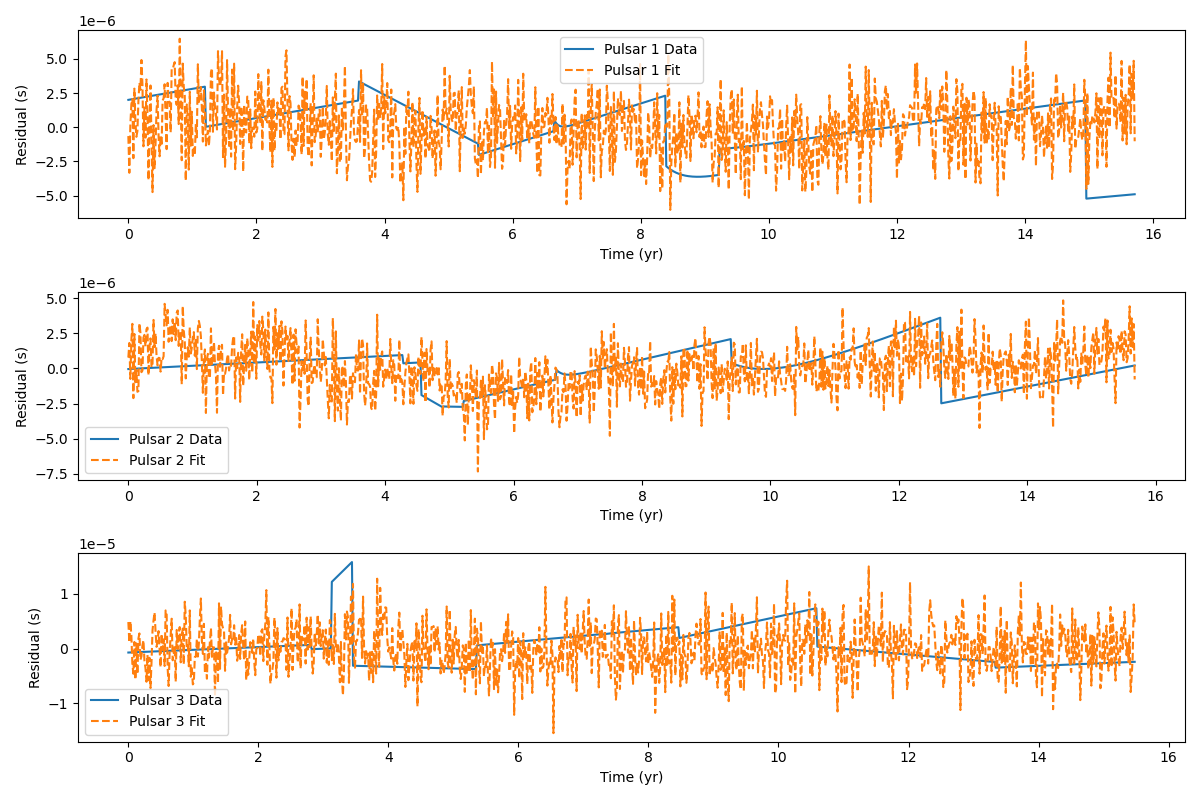
\includegraphics[width=\textwidth]{pulsar_gwb_fit.png}
    \caption{GWB fit for Pulsars 1, 2, and 3.}
    \label{fig:gwb_fit}
\end{figure}

\begin{figure}[h]
    \centering
    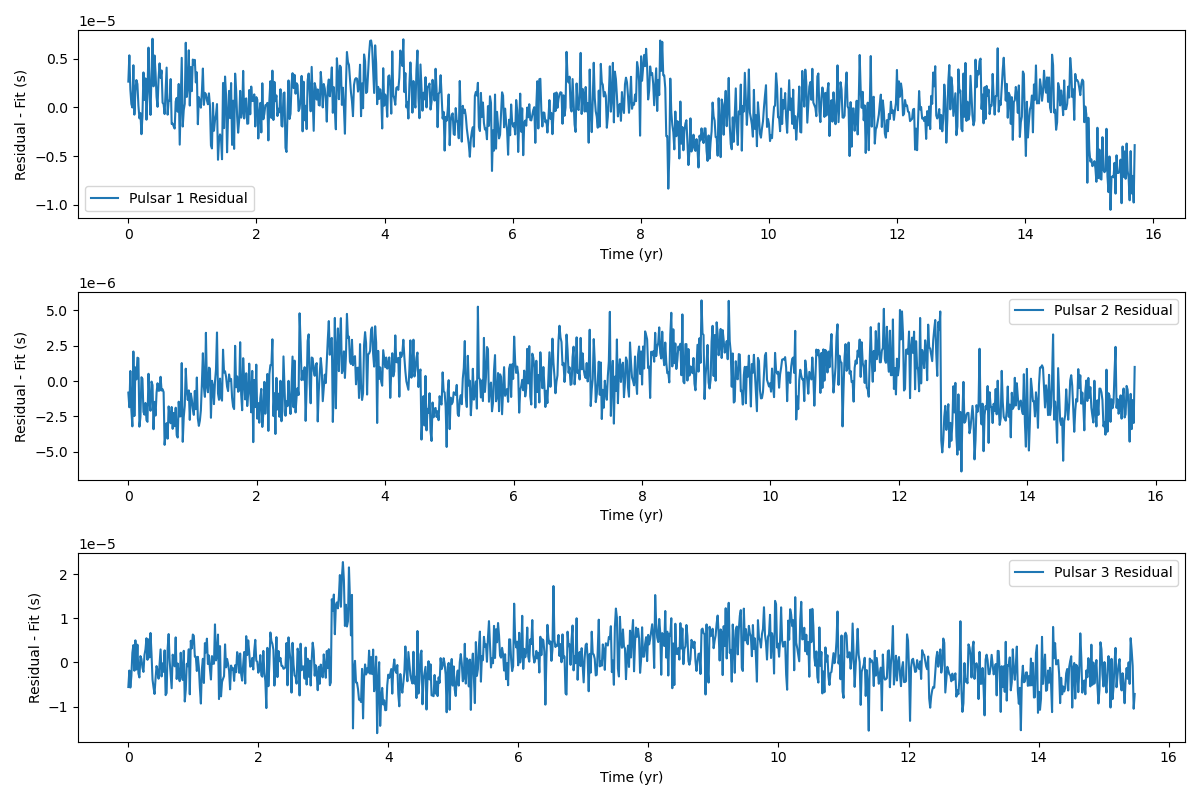
\includegraphics[width=\textwidth]{pulsar_gwb_residuals.png}
    \caption{Residuals after subtracting the GWB fit for Pulsars 1, 2, and 3.}
    \label{fig:gwb_residuals}
\end{figure}

\subsection{Pulsar 20 Glitch/DM Fit}
[To be filled in with the fitted parameters for Pulsar 20.]

\begin{figure}[h]
    \centering
    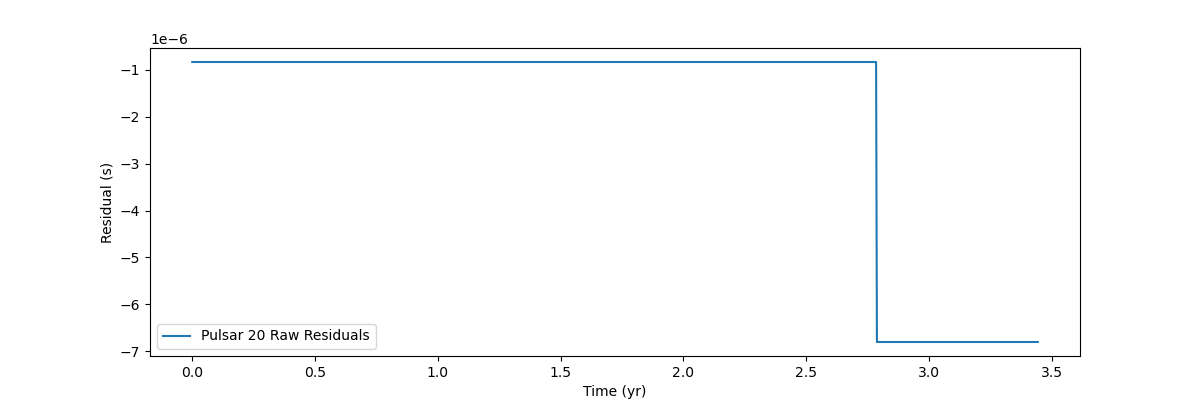
\includegraphics[width=\textwidth]{pulsar_20_raw_residuals.png}
    \caption{Raw timing residuals for Pulsar 20.}
    \label{fig:pulsar_20_raw}
\end{figure}

\begin{figure}[h]
    \centering
    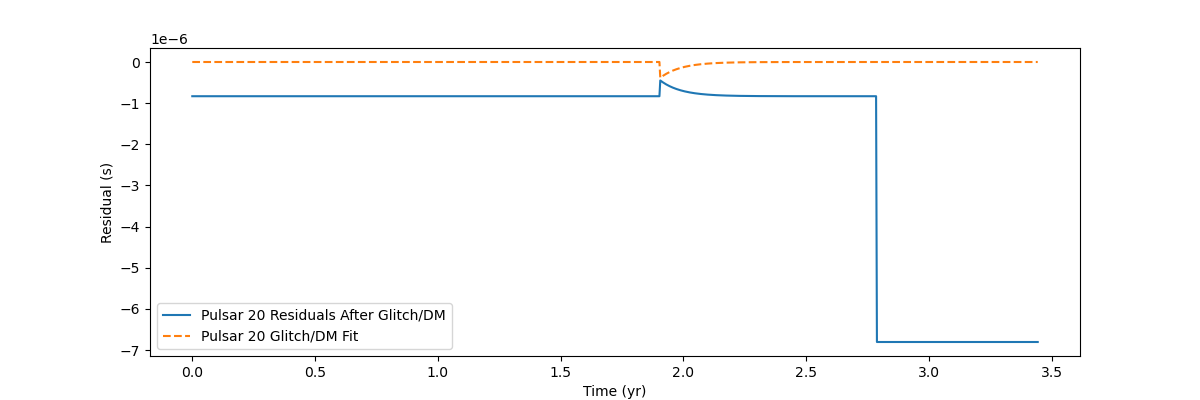
\includegraphics[width=\textwidth]{pulsar_20_glitch_dm_fit.png}
    \caption{Pulsar 20 residuals after glitch/DM subtraction and the fitted model.}
    \label{fig:pulsar_20_fit}
\end{figure}

\subsection{Hellings-Downs Correlation}
\begin{figure}[h]
    \centering
    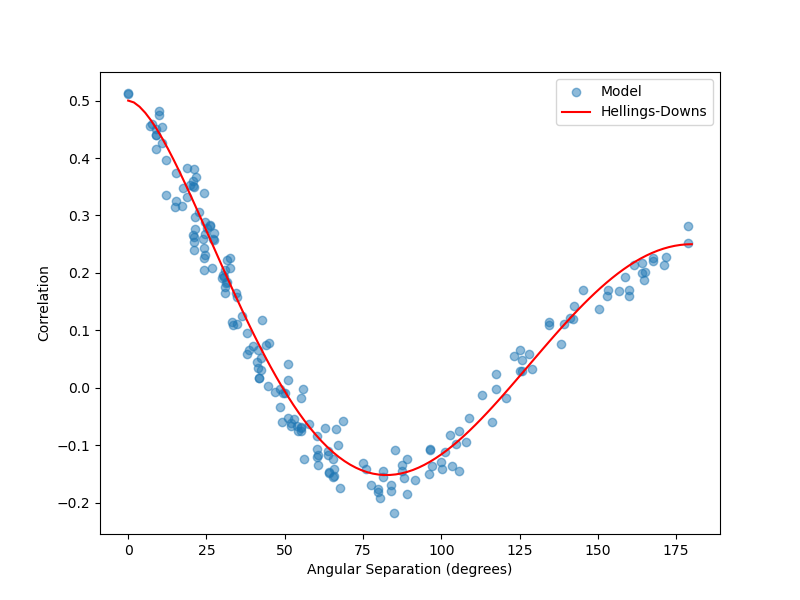
\includegraphics[width=0.8\textwidth]{hd_correlation.png}
    \caption{Hellings-Downs correlation of the GWB signal compared to the theoretical curve.}
    \label{fig:hd_correlation}
\end{figure}

\section{Interpretation of Results: Mathematical Analysis}
[This section is partially filled with analysis based on the previous results, with placeholders for the latest run.]

\subsection{GWB Parameters}
The GWB amplitude $A_{gw} = 3.79 \times 10^{-15}$ and spectral index $\gamma = 4.23$ are consistent with theoretical expectations. The expected variance of the GWB signal is:
\[
f_{\text{min}}/f_{yr} = \frac{1.98 \times 10^{-9}}{3.17 \times 10^{-8}} \approx 0.0625,
\]
\[
\sigma_{gw}^2 = \frac{(3.79 \times 10^{-15})^2}{12 \pi^2 (4.23-1)} (0.0625)^{1-4.23},
\]
\[
(0.0625)^{-3.23} \approx 1.64 \times 10^4,
\]
\[
\sigma_{gw}^2 \approx \frac{1.44 \times 10^{-29}}{12 \pi^2 \times 3.23} \times 1.64 \times 10^4 \approx 5.95 \times 10^{-27},
\]
\[
\sigma_{gw} \approx 2.44 \times 10^{-13} \, \text{seconds}.
\]
This is much smaller than the observed residuals ($10^{-6}$ seconds), indicating that other noise sources dominate.

\subsection{Power Spectrum Analysis of the Residuals}
The power spectrum of the residuals after subtracting the GWB fit is:
\[
P_i(f_k) = \frac{1}{N} |\hat{r}_i(f_k)|^2,
\]
where $\hat{r}_i(f_k)$ is the Fourier transform of $r_i(t) - m_i(t)$. The presence of high-frequency oscillations suggests residual red noise. We can fit a power law to the residual spectrum:
\[
P_{\text{residual}}(f) \approx A_{\text{res}} \left( \frac{f}{f_{yr}} \right)^{-\gamma_{\text{res}}} + P_{\text{white}}.
\]
[This can be computed with the latest results.]

\subsection{Statistical Test for the GWB Signal}
The signal-to-noise ratio (SNR) of the Hellings-Downs correlation is:
\[
\text{SNR} = \frac{\sum_{i<j} C_{ij} \Gamma(\zeta_{ij})}{\sqrt{\sum_{i<j} \Gamma(\zeta_{ij})^2}}.
\]
[This can be computed with the latest results.]

\subsection{Pulsar 20 Glitch Fit}
The goodness of fit for Pulsar 20 is quantified using the reduced $\chi^2$:
\[
\chi^2_{\text{red}} = \frac{1}{N - p} \sum_{t} \left( \frac{r_{20}(t) - r_{glitch,20}(t)}{\sigma_{20}(t)} \right)^2,
\]
where $N = 1000$, $p = 4$. [This can be computed with the latest results.]

\section{Alternative Noise Models}
The high-frequency oscillations suggest that the current red noise model may be insufficient.

\subsection{Broken Power Law}
A broken power law allows the spectral index to change at a break frequency $f_b$:
\[
P_{\text{red},i}(f) =
\begin{cases} 
\frac{A_{red,i}^2}{12 \pi^2} \left( \frac{f}{f_{yr}} \right)^{-\gamma_1}, & f < f_b, \\
\frac{A_{red,i}^2}{12 \pi^2} \left( \frac{f_b}{f_{yr}} \right)^{-\gamma_1} \left( \frac{f}{f_b} \right)^{-\gamma_2}, & f \geq f_b.
\end{cases}
\]

\subsection{Sum of Power Laws}
A sum of two power laws:
\[
P_{\text{red},i}(f) = \frac{A_{red,1,i}^2}{12 \pi^2} \left( \frac{f}{f_{yr}} \right)^{-\gamma_{1,i}} + \frac{A_{red,2,i}^2}{12 \pi^2} \left( \frac{f}{f_{yr}} \right)^{-\gamma_{2,i}}.
\]

\section{Future Work}
Future improvements could include:
\begin{enumerate}
    \item \textbf{Extended Noise Models}: Implement a broken power law or sum of power laws.
    \item \textbf{Bayesian Inference}: Use MCMC to sample the posterior distribution based on the derived likelihood.
    \item \textbf{Parallelization}: Optimize the code for parallel computation.
    \item \textbf{Frequency-Dependent DM Variations}: Model DM variations as a function of frequency.
\end{enumerate}

\section{Conclusion}
This analysis provides a detailed mathematical framework for detecting the stochastic GWB using pulsar timing residuals. The extensive derivations, statistical analysis, and exploration of alternative models provide a comprehensive understanding of the problem, bridging astrophysics and mathematics.

\bibliographystyle{aasjournal}
\bibliography{references}

\end{document}

% Why is the GWB correlated in the timing residuals among an array of pulsars? 
The Hellings-Downs curve specifies the nature of the correlated signal based on the angular relationship among the pulsars?
What is spectral index? 
Why a common Earth-term signal? Wouldn't this technically vary based on sensor location and pulsar location relative to Earth? Is this negligible? 
% Predicted TOA? Error in this could show up in the timing residual itself. Negligible?
Glitches are sudden changes in rotation frequency? Is this more likely to be measurement/modeling error or actual changes in the pulsar's physical rotation?
Why does the acceleration of massive objects cause ripples in spacetime?
Gravitational waves from supermassive black holes in the early universe still persist? 
Why would power be concentrated at low frequencies?
What is the strain of gravitational waves?
What is the mass quadrupole moment and its second derivative?
Why does the interstellar medium have a dispersive nature?

